\section{Baseline results}

\subsection{Generated fields}

The qualitative reference for the direct image-space diffusion model is given
in Figure~\ref{fig:ch5_baseline_sgm_comparison}, which compares one original
RTI density field with a reproducible $4\times4$ panel of unconditional SGM
samples. The generated fields reproduce the characteristic RTI interface
topology, including bubbles, spikes, and multi-mode roll-up. This visual
baseline is useful when interpreting the distributional scores below: the
evaluation concerns the generated ensemble, not a pointwise reconstruction of
the DNS fields.

\begin{figure}[H]
    \centering

    \begin{subfigure}[c]{0.48\textwidth}
        \centering
        
\includegraphics[width=\textwidth]{figures/ch5/original.png}
        \caption{Original RTI density field.}
        \label{fig:ch5_baseline_original}
    \end{subfigure}
    \hfill
    \begin{subfigure}[c]{0.48\textwidth}
        \centering
        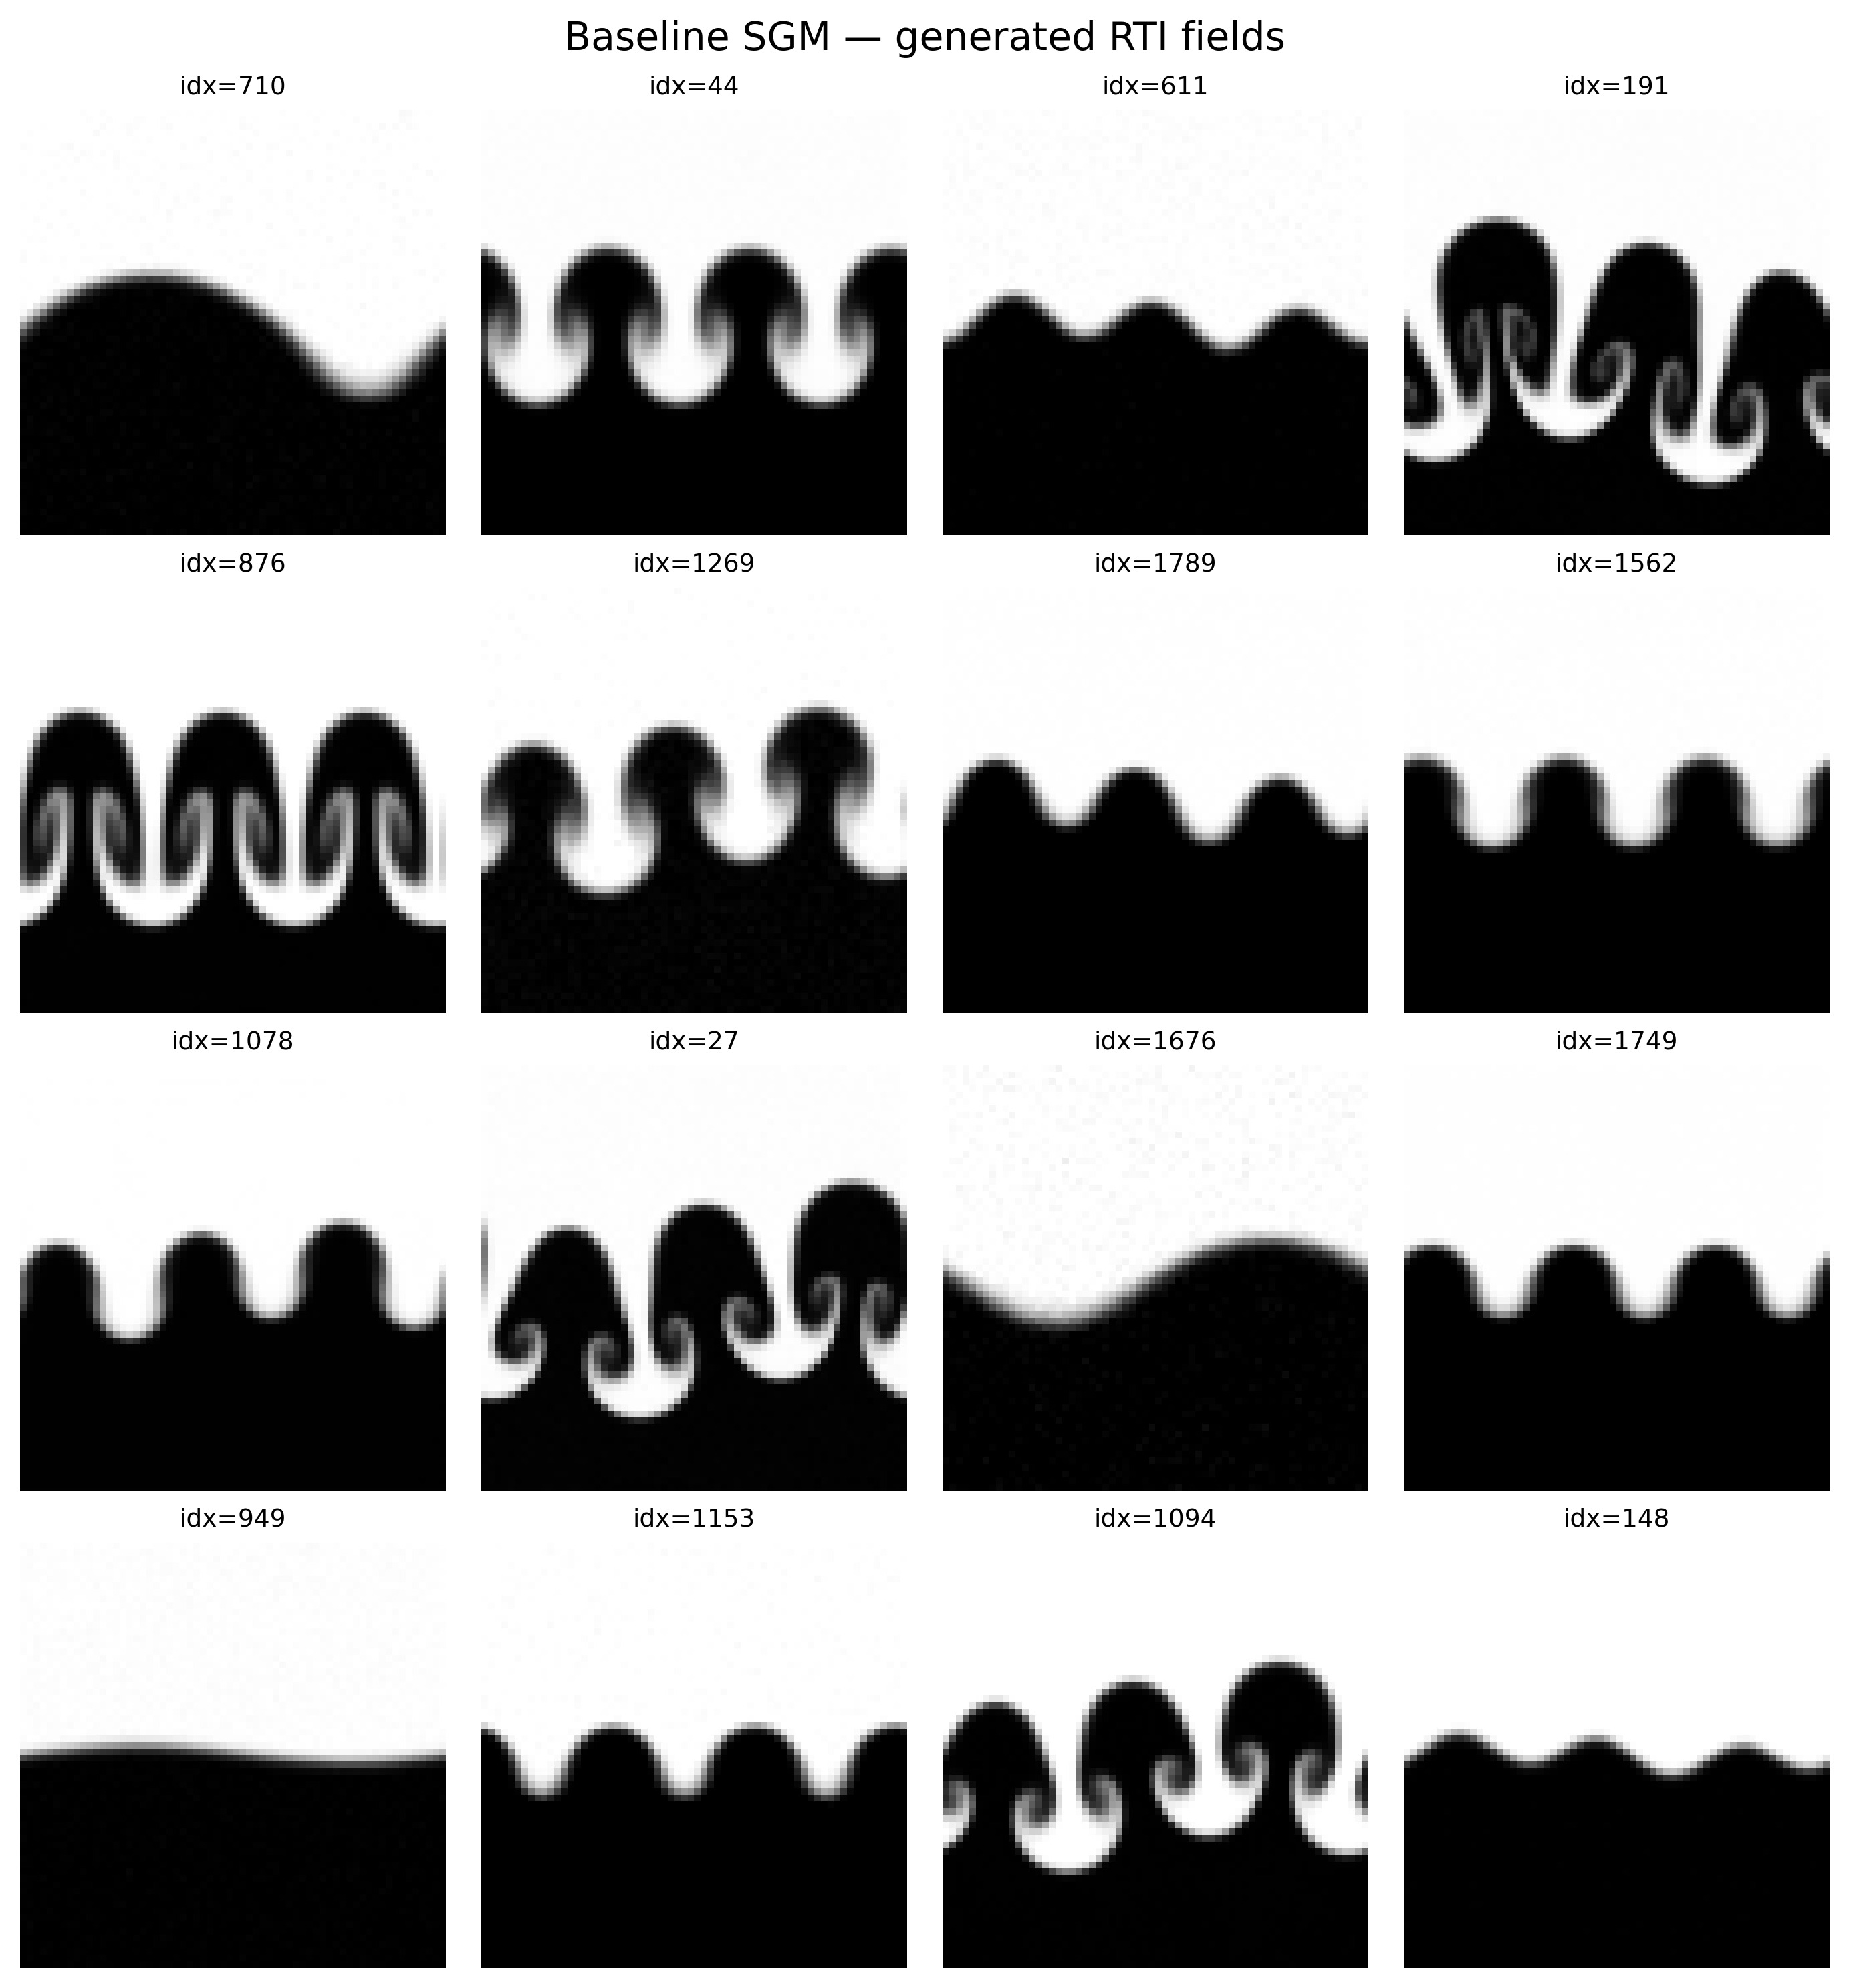
\includegraphics[width=\textwidth]{figures/ch5/baseline_sgm_grid.png}
        \caption{RTI density fields generated by the direct image-space SGM.}
        \label{fig:ch5_baseline_grid}
    \end{subfigure}

    \caption{Comparison between an original RTI density field (a) and samples generated by the baseline image-space SGM (b).}
    \label{fig:ch5_baseline_sgm_comparison}
\end{figure}

\subsection{PhyFID and FID comparison}

The notebook compares several datasets on 1000 images: a held-out part of the
validation set, a training subset, the generated SGM samples, pure-noise
samples produced by an untrained model, and an unrelated MNIST dataset used as
a negative control. The obtained scores are reported in
Table~\ref{tab:fid_phyfid_baseline}.

\begin{table}[H]
    \centering
    \begin{tabular}{lcc}
        \hline
        Comparison & PhyFID & FID Inception \\
        \hline
        val vs val & 0.021 & 0.0013 \\
        val vs train & 0.023 & 0.0008 \\
        val vs generated & 0.132 & 0.134 \\
        val vs noise & 6.04 & 42.05 \\
        val vs MNIST & 4.26 & 14.27 \\
        \hline
    \end{tabular}
    \caption{Comparison of validation, training, generated, noise and MNIST
    datasets using PhyFID and classical FID on 1000 images. Lower values are
    better.}
    \label{tab:fid_phyfid_baseline}
\end{table}

Several conclusions can be drawn from these values. First, the two reference
comparisons `val vs val` and `val vs train` give very low distances. This is
expected and confirms that both metrics behave consistently when comparing
datasets drawn from the same RTI distribution.

Second, the generated dataset remains significantly closer to the validation
set than pure noise or MNIST. In PhyFID space, the score for `val vs generated`
is approximately two orders of magnitude smaller than `val vs noise`
($0.1315$ versus $6.0399$). The same qualitative trend is observed with the
classical FID, where `val vs generated` remains small compared with
`val vs noise` and `val vs MNIST`.

These results indicate that the baseline SGM has learned non-trivial
statistical information about the RTI fields. The generated samples are clearly
not random images and it is therefore reasonable to continue the evaluation with 
other architectures and metrics.

\subsection{Line profile and spectral indicators}

The profiles and spectra extracted from the validation, generated and noise datasets are shown in Figures~\ref{fig:ch5_baseline_line_statistics} and
\ref{fig:ch5_baseline_energy_spectrum}. The corresponding distances are then reported in Table~\ref{tab:line_profile_spectrum_baseline}.

\begin{figure}[H]
    \centering
    
\includegraphics[width=0.90\textwidth]{figures/ch4/skewnorm_joyplot.png}
    \caption{Line-wise density statistics extracted from the validation,
    generated and noise datasets. The skew-normal fits emphasize the vertical
    organization of the fields and the contrast between physical samples and
    pure noise.}
    \label{fig:ch5_baseline_line_statistics}
\end{figure}

\begin{figure}[H]
    \centering
    
\includegraphics[width=0.90\textwidth]{figures/ch4/skewnorm_joyplot_energy_spectrum.png}
    \caption{Same comparison applied to the fluctuation energy spectrum. The
    generated samples remain much closer to the validation set than pure noise,
    but the spectral variability is still harder to match than the mean line
    profile.}
    \label{fig:ch5_baseline_energy_spectrum}
\end{figure}

\begin{table}[H]
    \centering
    \begin{tabular}{lcc}
        \hline
        Comparison & mean & fluctuation energy spectrum \\
        \hline
        val vs val & 0 & 0 \\
        val vs generated & 0.49 & 0.298 \\
        val vs noise & 13.1 & 1.66 \\
        val vs MNIST & 10.7 & 0.735 \\
        \hline
    \end{tabular}
    \caption{Comparison of validation, generated, noise and MNIST datasets using line-wise mean profile and fluctuation energy spectrum distances on 1000 images. Lower values are better.}
    \label{tab:line_profile_spectrum_baseline}
\end{table}

The results confirm the conclusions drawn from the feature-space metrics. The generated samples are much closer to the validation set than pure noise or MNIST, both in terms of mean vertical profile and fluctuation energy spectrum, by approximately two orders of magnitude.
